% Supplement subsections and tables typed below as "Section~S<n>.<m>" and "Table~S<n>"; build.sh checks each number
% against the built supplement.
% supplement-ref supp:angle=S1.6
% supplement-ref supp:settings=S2.4
% supplement-ref supp:statistics=S2.5
% supplement-ref supp:selection=S3.1
% supplement-ref supp:benchmark=S3.2
% supplement-ref supp:training=S3.3
% supplement-ref supp:sorting=S3.4
% supplement-ref supp:motion=S3.6
% supplement-ref supp:controlled=S3.7
% supplement-ref supp:ablation-arrowflow=S4.1
% supplement-ref supp:datasets=S5.2
% supplement-ref supp:learned-development=S6.2
% supplement-ref supp:learned-nested=S6.3
% supplement-ref supp:learned-swap=S6.4
% supplement-ref tab:s-motion-scramble=S28
% supplement-ref tab:s-motion-purity=S29
\section{Results}\label{sec:experiments}

The experiments ask six questions.
\begin{enumerate}[leftmargin=2em,topsep=2pt,itemsep=1pt]
\item How accurate is ArrowFlow next to standard classifiers tuned in the same way?
\item Does training the ranking filters help, compared with leaving them in their random starting orders?
\item What does each part of the method contribute?
\item Is it the particular signal sent down from the output layer that helps, or would any movement of the filters do?
\item What does training change inside the network, and where does its benefit stop?
\item Can motions of the same kind train a real-valued encoder network, and does ArrowFlow gain from it?
\end{enumerate}

In brief, ArrowFlow trails the best tuned classical model on all seventeen datasets, and training adds only a modest gain. The signal that training sends down does carry information. Yet a fixed kernel on rankings from the same encoder family is more accurate on most datasets. So the paper's contribution is the learning rule itself. Motions of the same kind also train a real-valued encoder network. With the trained encoder, ArrowFlow has the higher mean accuracy on 11 of the 17 datasets, significantly on one.

\subsection{How We Tested}\label{sec:protocol}

A fair test needs two things. It needs datasets that did not shape the method, and it needs a way of choosing settings that never looks at the test data. Section~S2.5 gives the complete protocol. The author used generative artificial intelligence tools for software development, running and analyzing the experiments, and editing the manuscript, and reviewed all of their output. The tools were Claude Opus 5, Claude Opus 5.5, Claude Fable 5 and Claude Fable 5.1 (Anthropic), and GPT 5.6 Sol and GPT 6 Astra (OpenAI).

\paragraph{Datasets.} We use seventeen classification datasets. Seven are standard benchmarks from the University of California, Irvine (UCI) Machine Learning Repository \citep{dua2019uci}, and they served during the method's development. They are Iris \citep{uci_iris}, Wine \citep{uci_wine}, Breast cancer \citep{uci_wdbc}, Wine quality (red wines, three quality classes) \citep{uci_winequality}, Vehicle \citep{uci_vehicle}, Segment \citep{uci_segment} and Digits \citep{uci_digits}. Wine quality's three classes are the quality scores 5 or less, 6, and 7 or more. The other ten, the further datasets, were fixed in advance as every dataset of a predefined pool of OpenML datasets \citep{vanschoren2014openml,bischl2021openml} that met prespecified eligibility rules, as interpreted during selection and before any model was fitted (Section~S3.1). They are balance-scale \citep{uci_balance}, mfeat-zernike \citep{uci_mfeat}, ionosphere \citep{uci_ionosphere}, vertebra-column \citep{uci_vertebral}, diabetes \citep{smith1988diabetes}, banknote-authentication \citep{uci_banknote}, qsar-biodeg \citep{uci_qsar}, steel-plates-fault \citep{uci_steel}, climate-model-simulation-crashes \citep{uci_climate} and the hepatitis C virus (HCV) data \citep{uci_hcv}. The method, its candidate settings and the comparison models were fixed before these ten were selected, and none of the ten had been used in the method's earlier development (Section~S5). The encoder network of Section~\ref{sec:learned-encoder} is an exception. Its target conversion and settings were developed on single splits of twelve of the seventeen datasets, six of them further datasets (Section~S6.2). All seventeen are small: 150 to 2,310 rows, 4 to 64 features and 2 to 10 classes (Section~S5.2).

\paragraph{How settings are chosen.} Every tuned setting is chosen by nested cross-validation, so within a run the test data never influence a choice. Each dataset is split into five parts that keep its class proportions. Each part serves once as the test set, and the split is repeated three times with different shuffles. So every model is tested on the same 15 test sets, called outer folds. All tuning happens inside the other four parts of each split, its training partition \citep{cawley2010selection}. These are split again into three inner folds, and each model picks its configuration there from at most 24 candidates. A stochastic model, one whose fit depends on a random seed, has its three best candidates rescored with all three fitting seeds. The chosen configuration is refitted on the whole training partition and scored once on the test set.

\paragraph{Models.} ArrowFlow always uses $K=7$ views, the nearest-neighbor readout and the validation checkpoint. Its 16 candidates vary the hidden-layer widths, the learning rate and two encoder settings (Section~S2.4). The comparison models are five scikit-learn classifiers \citep{pedregosa2011sklearn}, each tuned in the same way. They are a support vector classifier (SVC) with a radial basis function kernel, a random forest, a multilayer perceptron (MLP), numeric kNN on the standardized raw features and gradient boosting. The majority class gives a baseline. ArrowFlow also chooses its readout's neighbor count and weighting inside every fit, outside the candidate budget.

\paragraph{How differences are judged.} Errors are in percent and differences in percentage points (pp). Tables give each model's mean error over the 15 test sets, with its standard deviation (SD) across them. To compare two models, we take their accuracy difference on each test set and report the mean with a 95\% interval. The 15 splits share training data, so their differences are correlated. We use the corrected resampled $t$ interval, which is wider to allow for that \citep{nadeau2003inference,bouckaert2004evaluating}. Over many datasets some differences look large by chance alone. We therefore correct the $p$ values for the number of comparisons with the Holm method \citep{holm1979simple}, and a difference is significant when its corrected $p$ value is below $0.05$. Each correction covers a group of comparisons that a run protocol fixed before they were scored. Each such protocol was frozen before its run, with its hash and time recorded, but none was deposited with an external registry. Analyses defined afterwards are exceptions, and we call them post hoc. On the seven benchmark datasets, the training comparisons were fixed after ArrowFlow's own results there were known (Section~S2.5).

\subsection{How Accurate Is ArrowFlow?}\label{sec:main-benchmark}

How does ArrowFlow compare with standard classifiers that get the same data, the same folds and the same cap on candidates? Table~\ref{tab:main} gives the test error of every model on every dataset.

ArrowFlow is never the most accurate model. On every one of the seventeen datasets the best tuned classical model has lower error, by $0.19$ (banknote-authentication) to $5.32$ percentage points (ionosphere). Ranked within each dataset and averaged, ArrowFlow comes fourth of the six tuned models, between random forest and gradient boosting. On the ten further datasets alone it comes fifth, ahead of numeric kNN only (Section~S3.2). Accuracy can hide a weakness on a rare class. Balanced accuracy averages, over the classes, the share of each class's rows that a model gets right. On climate-model-simulation-crashes, ArrowFlow's balanced accuracy is 51.2 percent, barely above the 50 percent of the majority class. The support vector classifier reaches 76.1 percent (Section~S3.2).

% Rendered by render_tables.py from run files; do not edit by hand.
\begin{sidewaystable}[p]
\caption{\textbf{ArrowFlow against five tuned classical models and the majority class on the seventeen datasets.} Mean test error in percent over the 15 outer folds (5 folds $\times$ 3 repeats), with the standard deviation (SD) across folds in parentheses; the SD describes spread, not a confidence interval. Every model chose its configuration on inner folds only (Section~\ref{sec:protocol}). Bold marks the lowest unrounded error among ArrowFlow and the five classical models. The last column gives ArrowFlow's error minus that of the best tuned classical model, the majority class excluded, in percentage points, positive when ArrowFlow trails; it is positive on all seventeen datasets. It is computed from unrounded errors, so it can differ in the last digit from the printed errors; Section~S3.2 lists the errors of the tuned models to two decimals. The marks are post hoc flags. c: the best tuned classical model has less than 1\% error. m: ArrowFlow is within 0.5 points of the majority class, and the best tuned model is at least 2 points better. n: no model has lower error than the majority class. SVC: support vector classifier with a radial basis function (RBF) kernel; MLP: multilayer perceptron; kNN: nearest-neighbor classifier; HCV: hepatitis C virus.}
\label{tab:main}
\centering
\scriptsize
\setlength{\tabcolsep}{3pt}
\resizebox{\ifdim\width>\linewidth\linewidth\else\width\fi}{!}{%
\begin{tabular}{lrrrrrrrr}
\toprule
Dataset & ArrowFlow & SVC (RBF) & Random forest & MLP & Numeric kNN & \begin{tabular}[b]{@{}r@{}}Gradient\\boosting\end{tabular} & \begin{tabular}[b]{@{}r@{}}Majority\\class\end{tabular} & \begin{tabular}[b]{@{}r@{}}Gap to best\\tuned (pp)\end{tabular} \\
\midrule
\multicolumn{9}{l}{\emph{Benchmark datasets}} \\
Iris & 5.0 (3.5) & \textbf{4.0 (3.4)} & 5.3 (4.3) & 4.1 (3.7) & 4.7 (3.3) & 5.6 (3.5) & 66.7 (0.0) & +1.04 \\
Wine & 3.2 (2.9) & \textbf{1.5 (2.3)} & 1.8 (1.6) & 1.9 (2.2) & 3.4 (3.4) & 2.6 (2.5) & 60.1 (1.6) & +1.69 \\
Breast cancer & 2.7 (1.1) & \textbf{2.3 (1.5)} & 4.3 (1.5) & 2.9 (1.5) & 3.5 (1.5) & 3.9 (1.6) & 37.3 (0.4) & +0.33 \\
Wine quality & 27.7 (2.1) & 33.1 (3.4) & \textbf{27.2 (2.3)} & 32.3 (2.6) & 28.8 (2.2) & 30.7 (2.1) & 53.5 (0.1) & +0.47 \\
Vehicle & 19.9 (1.5) & \textbf{16.5 (2.0)} & 25.7 (2.3) & 17.2 (2.0) & 29.3 (2.6) & 24.3 (2.2) & 74.2 (0.3) & +3.40 \\
Segment & 2.6 (0.7) & 3.3 (0.9) & \textbf{1.9 (0.7)} & 2.8 (0.9) & 3.4 (1.1) & 2.1 (0.6) & 85.7 (0.0) & +0.66 \\
Digits & 2.8 (0.9) & \textbf{1.8 (0.6)} & 2.4 (0.7) & 2.3 (0.8) & 2.1 (0.7) & 3.3 (0.9) & 89.9 (0.2) & +0.97 \\
\midrule
\multicolumn{9}{l}{\emph{Further datasets}} \\
balance-scale & 6.0 (1.3) & \textbf{2.1 (1.8)} & 13.8 (2.1) & 2.2 (1.1) & 10.2 (1.5) & 8.4 (0.8) & 54.2 (0.3) & +3.95 \\
mfeat-zernike & 19.3 (1.0) & \textbf{17.1 (1.6)} & 22.3 (2.0) & 18.9 (1.2) & 19.6 (1.7) & 22.4 (1.8) & 90.0 (0.0) & +2.18 \\
ionosphere & 11.2 (3.4) & \textbf{5.9 (2.7)} & 7.0 (2.5) & 8.0 (2.6) & 10.2 (3.5) & 6.6 (2.1) & 35.9 (0.4) & +5.32 \\
vertebra-column & 16.9 (3.6) & \textbf{14.0 (5.2)} & 15.8 (3.2) & 15.4 (4.4) & 19.8 (4.0) & 17.8 (4.3) & 51.6 (0.0) & +2.90 \\
diabetes & 24.0 (2.5) & \textbf{22.7 (2.9)} & 23.9 (2.6) & 23.5 (1.5) & 24.5 (2.7) & 24.0 (3.2) & 34.9 (0.2) & +1.34 \\
banknote-authentication$^{\mathrm{c}}$ & 0.2 (0.5) & 0.0 (0.1) & 0.9 (0.7) & \textbf{0.0 (0.0)} & 0.3 (0.5) & 0.3 (0.3) & 44.5 (0.1) & +0.19 \\
qsar-biodeg & 12.6 (1.8) & 12.2 (3.1) & 13.0 (2.1) & \textbf{12.0 (2.9)} & 13.7 (2.7) & 13.2 (2.5) & 33.7 (0.2) & +0.52 \\
steel-plates-fault & 24.8 (1.5) & 23.9 (2.1) & 21.2 (1.6) & 24.2 (1.7) & 25.5 (1.4) & \textbf{21.0 (1.8)} & 65.3 (0.1) & +3.82 \\
climate-model-simulation-crashes$^{\mathrm{m}}$ & 8.3 (0.6) & \textbf{5.4 (2.2)} & 6.4 (1.1) & 5.6 (1.7) & 6.8 (1.1) & 5.9 (1.4) & 8.5 (0.4) & +2.96 \\
HCV$^{\mathrm{n}}$ & 75.6 (1.7) & 75.5 (2.0) & 75.9 (1.6) & 75.0 (1.8) & \textbf{74.1 (2.6)} & 76.9 (2.4) & 73.9 (0.2) & +1.50 \\
\bottomrule
\end{tabular}
}
\end{sidewaystable}


\subsection{Does Training Help?}\label{sec:training-controls}

Random ranking filters already turn an input into a new ranking, and the nearest-neighbor readout may work well on it without any training. To see what the learning rule adds, we compare ArrowFlow with two controls that train no filters but are otherwise tuned exactly like it (Table~\ref{tab:training}). The untrained ArrowFlow keeps its random initial filters. Tuned input footrule kNN skips the ranking layers and applies the nearest-neighbor readout directly to the encoded input rankings.

% Rendered by render_tables.py from run files; do not edit by hand.
\begin{table}[!htbp]
\caption{\textbf{What training adds, on the seventeen datasets.} Upper part: mean test error in percent, lower is better, of five classifiers that all predict from nearest neighbors. From left to right they are numeric kNN on the standardized raw features, numeric kNN on the projected scores before sorting, tuned input footrule kNN on the encoded input rankings, the untrained ArrowFlow and ArrowFlow. Neighboring columns differ in more than one component, so this ladder describes and does not decompose. Lower part: ArrowFlow's accuracy minus that of each control in percentage points, positive when ArrowFlow is more accurate, with its 95\% interval, which is not corrected for multiple comparisons. Holm $p$ is corrected over the comparisons named in the block header, which the run protocols fixed before the controls were scored; the benchmark family was fixed after ArrowFlow's own benchmark results were known. $^\ddagger$: still below 0.05 after one post hoc correction over all 34 comparisons. Both controls share ArrowFlow's encoder family but choose their own settings on inner folds. kNN: nearest-neighbor classifier; HCV: hepatitis C virus.}
\label{tab:training}
\centering
\scriptsize
\setlength{\tabcolsep}{3pt}
\begin{tabular}{lrrrrr}
\toprule
Dataset & \begin{tabular}[b]{@{}r@{}}Numeric kNN,\\raw features\end{tabular} & \begin{tabular}[b]{@{}r@{}}Numeric kNN,\\projected scores\end{tabular} & \begin{tabular}[b]{@{}r@{}}Tuned input\\footrule kNN\end{tabular} & \begin{tabular}[b]{@{}r@{}}Untrained\\ArrowFlow\end{tabular} & ArrowFlow \\
\midrule
\multicolumn{6}{l}{\emph{Benchmark datasets}} \\
Iris & 4.7 & 4.0 & 5.6 & 6.0 & 5.0 \\
Wine & 3.4 & 3.9 & 4.9 & 3.9 & 3.2 \\
Breast cancer & 3.5 & 3.3 & 3.6 & 3.2 & 2.7 \\
Wine quality & 28.8 & 28.2 & 28.1 & 27.8 & 27.7 \\
Vehicle & 29.3 & 25.1 & 24.7 & 23.4 & 19.9 \\
Segment & 3.4 & 3.6 & 3.8 & 3.6 & 2.6 \\
Digits & 2.1 & 2.4 & 2.8 & 3.0 & 2.8 \\
\midrule
\multicolumn{6}{l}{\emph{Further datasets}} \\
balance-scale & 10.2 & 10.3 & 10.9 & 11.0 & 6.0 \\
mfeat-zernike & 19.6 & 19.0 & 21.5 & 21.6 & 19.3 \\
ionosphere & 10.2 & 12.3 & 11.2 & 11.4 & 11.2 \\
vertebra-column & 19.8 & 16.7 & 17.8 & 18.0 & 16.9 \\
diabetes & 24.5 & 24.3 & 24.0 & 24.8 & 24.0 \\
banknote-authentication & 0.3 & 0.2 & 0.1 & 0.2 & 0.2 \\
qsar-biodeg & 13.7 & 13.8 & 14.0 & 13.5 & 12.6 \\
steel-plates-fault & 25.5 & 25.4 & 25.2 & 25.6 & 24.8 \\
climate-model-simulation-crashes & 6.8 & 7.6 & 8.3 & 8.4 & 8.3 \\
HCV & 74.1 & 75.6 & 75.7 & 75.2 & 75.6 \\
\bottomrule
\end{tabular}
\par\medskip
\begin{tabular}{lrrrr}
\toprule
Dataset & \begin{tabular}[b]{@{}r@{}}ArrowFlow $-$\\untrained (pp)\end{tabular} & \begin{tabular}[b]{@{}r@{}}Holm\\$p$\end{tabular} & \begin{tabular}[b]{@{}r@{}}ArrowFlow $-$ tuned\\input footrule kNN (pp)\end{tabular} & \begin{tabular}[b]{@{}r@{}}Holm\\$p$\end{tabular} \\
\midrule
\multicolumn{5}{l}{\emph{Benchmark datasets: Holm correction over fourteen comparisons}} \\
Iris & +0.96 [$-$1.35, +3.28] & 1.000 & +0.52 [$-$2.25, +3.29] & 1.000 \\
Wine & +0.74 [$-$1.13, +2.61] & 1.000 & +1.68 [$-$1.04, +4.40] & 1.000 \\
Breast cancer & +0.55 [$-$0.44, +1.53] & 1.000 & +0.88 [$-$0.10, +1.86] & 0.751 \\
Wine quality & +0.11 [$-$1.44, +1.66] & 1.000 & +0.44 [$-$1.23, +2.10] & 1.000 \\
Vehicle & +3.51 [+1.27, +5.74] & 0.060 & +4.81 [+1.86, +7.75] & 0.049 \\
Segment & +1.06 [+0.24, +1.88] & 0.161 & +1.18 [+0.39, +1.97] & 0.075 \\
Digits & +0.22 [$-$0.70, +1.13] & 1.000 & $-$0.03 [$-$1.01, +0.96] & 1.000 \\
\midrule
\multicolumn{5}{l}{\emph{Further datasets: Holm correction over ten comparisons per control}} \\
balance-scale & +4.98 [+3.38, +6.57] & $<$0.001$^\ddagger$ & +4.91 [+2.98, +6.83] & $<$0.001$^\ddagger$ \\
mfeat-zernike & +2.34 [+1.28, +3.40] & 0.003$^\ddagger$ & +2.18 [+1.09, +3.28] & 0.007$^\ddagger$ \\
ionosphere & +0.16 [$-$3.60, +3.92] & 1.000 & $-$0.00 [$-$2.97, +2.97] & 1.000 \\
vertebra-column & +1.08 [$-$2.43, +4.58] & 1.000 & +0.97 [$-$1.52, +3.46] & 1.000 \\
diabetes & +0.71 [$-$1.59, +3.01] & 1.000 & $-$0.03 [$-$1.52, +1.47] & 1.000 \\
banknote-authentication & +0.03 [$-$0.25, +0.31] & 1.000 & $-$0.09 [$-$0.68, +0.50] & 1.000 \\
qsar-biodeg & +0.92 [$-$0.14, +1.97] & 0.663 & +1.42 [+0.45, +2.39] & 0.056 \\
steel-plates-fault & +0.72 [$-$1.23, +2.67] & 1.000 & +0.39 [$-$1.31, +2.08] & 1.000 \\
climate-model-simulation-crashes & +0.02 [$-$0.43, +0.48] & 1.000 & $-$0.04 [$-$0.65, +0.57] & 1.000 \\
HCV & $-$0.37 [$-$2.59, +1.86] & 1.000 & +0.13 [$-$2.73, +2.99] & 1.000 \\
\bottomrule
\end{tabular}
\end{table}


Training helps, but modestly. ArrowFlow is more accurate than the untrained ArrowFlow on 16 of the 17 datasets. A post hoc one-sided signed-rank test supports the gain over all seventeen ($p<0.001$) and over the ten further datasets alone ($p=0.007$; Section~S3.3). This test ranks the differences across datasets by size and asks whether the positive ones outweigh the negative ones more than chance allows \citep{demsar2006statistical}. Yet the untrained version comes within one percentage point on 12 of the 17. The gain is significant against at least one control on three datasets: Vehicle, against tuned input footrule kNN, and balance-scale and mfeat-zernike, against both controls. Only the last two survive a stricter, post hoc correction over all 34 comparisons (Section~S3.3). Table~\ref{tab:training} also checks whether sorting itself helps. On the seven benchmark datasets, sorting the projected scores made no detectable difference to a nearest-neighbor readout (Section~S3.4). On the ten further datasets, where the comparison is descriptive, sorting raised the readout's error on six of them, by up to 2.5 points.

One prespecified test asks where training helps most. Before the runs, four further datasets, balance-scale, mfeat-zernike, ionosphere and vertebra-column, were marked because the published results we counted \citep{vanschoren2014openml,fernandezdelgado2014hundreds} put tuned kNN at least 5 percentage points behind the best tuned model (Section~S3.1). Training gained more on these four than on the other six ($p=0.033$). But by construction these datasets also leave nearest neighbors more room to improve. So the test cannot tell whether training helps where nearest neighbors suit the raw features poorly, or simply where there is more to gain. It also rests on only ten datasets, and without the three datasets that Table~\ref{tab:main} flags it gives $p=0.20$, a post hoc check (Section~S3.3).

\subsection{What Does Each Part Contribute?}\label{sec:components}

ArrowFlow combines several parts: the nearest-neighbor readout, seven views, a validation checkpoint and augmentation. To see what each contributes, we remove or replace one part at a time and keep everything else, including the configuration ArrowFlow chose on each split.

The readout makes the largest difference. Predicting with the prototype readout, the nearest output filter, instead of the nearest stored training examples is less accurate on 16 of the 17 datasets, by more than one percentage point on eight of them. Seven views are more accurate than the first, target-aware view alone on 12 of the 17. Removing the checkpoint or augmentation changes mean accuracy by less than $0.2$ percentage points. These configurations were chosen for ArrowFlow's own readout, so the comparison with the prototype readout favors ArrowFlow (Section~S4.1).

\subsection{Is It the Signal That Helps?}\label{sec:motion-controls}

Training might help simply because it moves the filters, whatever the direction. To test whether the particular signal is what helps, we keep everything else identical and tamper only with the motions that the output layer sends down to the hidden filters. We compare ArrowFlow with three controls.
\begin{itemize}[leftmargin=2em,topsep=2pt,itemsep=1pt]
\item With \emph{frozen filters}, the hidden filters stay in their random starting orders, and everything else is ArrowFlow's own, settings included (Section~S3.6).
\item With \emph{permuted alignment}, each motion is delivered to a filter of the same layer drawn at random, afresh in every batch.
\item With \emph{random directions}, the directions are shuffled among the motions, so a filter may be pushed away from an input it should approach.
\end{itemize}
The two scrambled controls keep the number of motions, their sizes and their total weight.

% Figure: matched motion-signal controls. Rendered by render_tables.py via render_figures.motion_forest from the
% motion-controls analysis outputs; nothing numeric is typed here.
% supplement-ref tab:s-motion-scramble=S28
% supplement-ref tab:s-motion-purity=S29
\begin{figure}[!htbp]
\centering
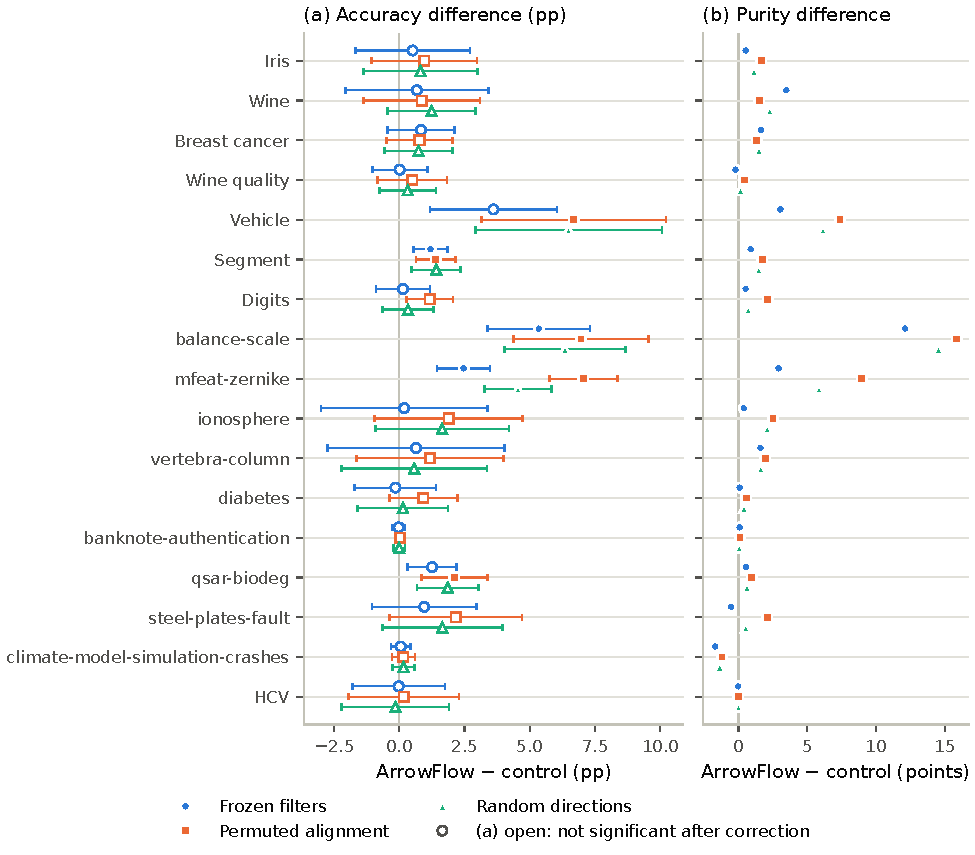
\includegraphics[width=0.92\textwidth]{figures/data/fig8_motion_forest.pdf}
\caption{\textbf{Is it the signal that helps?} (a)~ArrowFlow's accuracy minus that of each control, in percentage points, with 95\% intervals (not simultaneous); positive favors ArrowFlow. Frozen filters: the hidden filters never move. Permuted alignment: each motion reaches a filter of the same layer drawn at random, afresh in every batch. Random directions: the directions of the motions are shuffled. Both scrambled controls keep the number of motions, their sizes and their total weight. Filled marks in panel (a) remain significant after a Holm correction across the seventeen datasets within each control: 3 datasets for frozen filters, 5 for permuted alignment and 3 for random directions. The intervals are not adjusted for multiple comparisons, so an open mark's interval can exclude zero. In panel (a), ArrowFlow is more accurate than frozen filters on 14 of the 17 datasets, than permuted alignment on 17 and than random directions on 16. (b)~Neighborhood purity, how often an example's nearest training examples share its class: ArrowFlow minus each control, in percentage points, on the test rows; descriptive, with no interval and no test, so its marks carry no fill coding. ArrowFlow is purer than all three controls on 13 of the 17 datasets. In both panels, a scramble's mark to the right of the mark of frozen filters means that the scramble is less accurate than frozen filters, or in panel~(b) less pure. Tables~S28 and~S29 give these comparisons directly. HCV: hepatitis C virus.}
\label{fig:motion-forest}
\end{figure}


A scrambled signal leaves the network less accurate than no training at all. Delivering the motions to the wrong filters does so on 16 of the 17 datasets, and shuffling their directions on 14 of the 17. These counts are descriptive, but a post hoc one-sided signed-rank test across the datasets supports both ($p<0.001$; Table~S28). The neighborhoods that the readout uses degrade in the same way. We measure them by their purity, how often an example's nearest training examples share its class. On most datasets, an example's nearest training examples share its class less often after either scramble than with frozen filters (Figure~\ref{fig:motion-forest}b and Table~S29). So the motions carry information about which filter should move and in which direction. A permutation fixed for the whole of training, the analog of feedback alignment \citep{lillicrap2016random}, was not tested (Section~S3.6).

Figure~\ref{fig:motion-forest}a compares ArrowFlow itself with each control. Against frozen filters ArrowFlow is more accurate on 14 of the 17 datasets, fewer than the 16 against the untrained ArrowFlow of Section~\ref{sec:training-controls}, which chooses its own settings. The three exceptions lie within 0.2 points of zero, and the mean gain is about one point against either. The two scrambles differ in strength, so each is compared with frozen filters rather than with the other (Section~S3.6).

\subsection{What Training Does and Where It Stops}\label{sec:controlled}

The studies below look inside the trained networks and test the limits of the approach.

\paragraph{What does training teach the network?} One dataset makes this easy to see. In the balance-scale data, each example places a weight at some distance on each side of a balance. The task is to say whether the balance tips left, tips right or stays level. A level balance is rare, about one example in thirteen, and it is hard to spot, because it sits exactly on the line between the other two outcomes. Before training, ArrowFlow almost never recognizes a level balance, and neither do simpler nearest-neighbor methods on the same inputs. None of them gets more than 5 in 100 right. After training, ArrowFlow gets about half of them right. The two common outcomes are easy either way. ArrowFlow recognizes tips to either side nearly always, before training and after. So most of what training adds on this dataset comes from learning this one thin class. The support vector classifier recognizes nearly every level balance, far more often than ArrowFlow, so other methods can find this class too (Section~S3.7).

\paragraph{Do the filters move at all?} The validation checkpoint could, in principle, hand back the random starting filters. It never did. In none of the 1,785 trained views of one fitting seed did the checkpoint keep the initial filters, and in the networks with one hidden layer nearly every hidden filter ended in a new order. Ties limit what the layers can express, though. The distances from an input to many filters bunch together in a narrow band (Section~\ref{sec:theory-margin}). So two filters often sit at exactly the same distance from an input, and their IDs then decide their order. In a hidden layer of 128 filters that ranks 32 items, about four in five distances are shared with another filter, before training and after, as with random filters (Section~S3.7).

\paragraph{Does a second hidden layer help?} It did not. We refitted every split with one hidden layer of 128 filters and with two, of 64 and then 128 filters. Every other setting, including the 200 updates and the learning rate, was the one chosen for that split. On 185 of the 255 splits, that choice was made for a network with one hidden layer. With the earlier relay, one hidden layer was more accurate than two on 15 of the 17 datasets, although no difference was significant after correction. With the corrected relay, two layers were about as accurate as one, and a second layer still did not help (Section~S3.7). Over the datasets, two layers minus one averaged $-0.24$ points, with a post hoc 95\% interval from $-0.60$ to $+0.12$.

\paragraph{Does the voting rule make a difference?} Each update merges its votes by a weighted Borda count, one of the three exchangeable stages of Section~\ref{sec:arrow}. We replaced it in the hidden layers by the footrule median, the ranking with the smallest total footrule distance to the votes. Its prior weight, the weight of the filter's current order, was set once, on training data from two datasets, so that it moved the filters about as often as the Borda count there. Over all datasets it moves them less often, and per dataset the movement differs widely (Section~S3.7). The Borda count was more accurate on 13 of the 17 datasets, but significantly so only on Vehicle. This compares two voting rules and does not test Arrow's theorem (Section~S3.7).

\paragraph{Do established methods do as well?} Could an established method match ArrowFlow without any learned filters? On most datasets, yes. Take a support vector classifier with a fixed Kendall kernel \citep{jiao2015kernels,jiao2018kendall}. It compares two rankings by Kendall's $\tau$, the share of item pairs that they order alike minus the share that they order differently. Applied to rankings from ArrowFlow's own encoder, with its encoder settings chosen on its own inner folds, the classifier is more accurate than ArrowFlow on 14 of the 17 datasets. The angle property of Section~\ref{sec:theory-alphabet} suggests why. For a random view, the expected $\tau$ of two encoded rankings over the draw of the projection is $1-2\theta/\pi$, where $\theta$ is the angle between their expanded, standardized features (Section~S1.6). Up to a scale and a shift, this is the arc-cosine kernel of order zero \citep{cho2009kernel}, so the classifier acts much like a kernel machine on the features. ArrowFlow has a higher mean accuracy than nearest neighbors after a linear discriminant projection on 12 of the 17 datasets, and after a principal component projection on 11. After a learned metric (neighborhood components analysis), it has the higher mean accuracy on only 7 of the 17 (Section~S3.7).

\paragraph{Does training improve the representation itself?} ArrowFlow reads its hidden rankings with a nearest-neighbor vote. Training could improve the rankings themselves, or it could only arrange them to suit that vote. To tell the two apart, we read the untrained and the trained hidden rankings with a strong fixed readout, a support vector classifier with the same Kendall kernel. On the ten further datasets, the scope fixed in advance, the trained rankings had the higher mean accuracy on only 3, and no difference was significant. Over the ten datasets, trained minus untrained averaged $-0.10$ points, with a post hoc 95\% interval from $-0.56$ to $+0.35$. For this outcome, the protocol had fixed the following statement before the test. Training improves the nearest-neighbor neighborhoods but not the representation read by a strong fixed readout (Section~S3.7).

\subsection{Can the Ranking Signal Train the Encoder?}\label{sec:learned}

The motions have so far trained ranking filters. Here we ask whether they can also train the real-valued weights of the encoder network of Section~\ref{sec:learned-encoder}, and whether ArrowFlow gains from the trained encoder. The answer to the first is yes, and the answer to the second is a modest yes, by a rule fixed before the run (Figure~\ref{fig:learned}). Both studies below use the benchmark's test sets, but the target conversion and its settings were developed on single splits of twelve of its seventeen datasets (Section~\ref{sec:protocol}).

% Figure: the learned encoder. Rendered by render_tables.py via render_figures.encoder_forest from the run files of the
% two studies of the learned encoder; nothing numeric is typed here.
% supplement-ref supp:learned-swap=S6.4
% supplement-ref supp:learned-development=S6.2
\begin{figure}[!htbp]
\centering
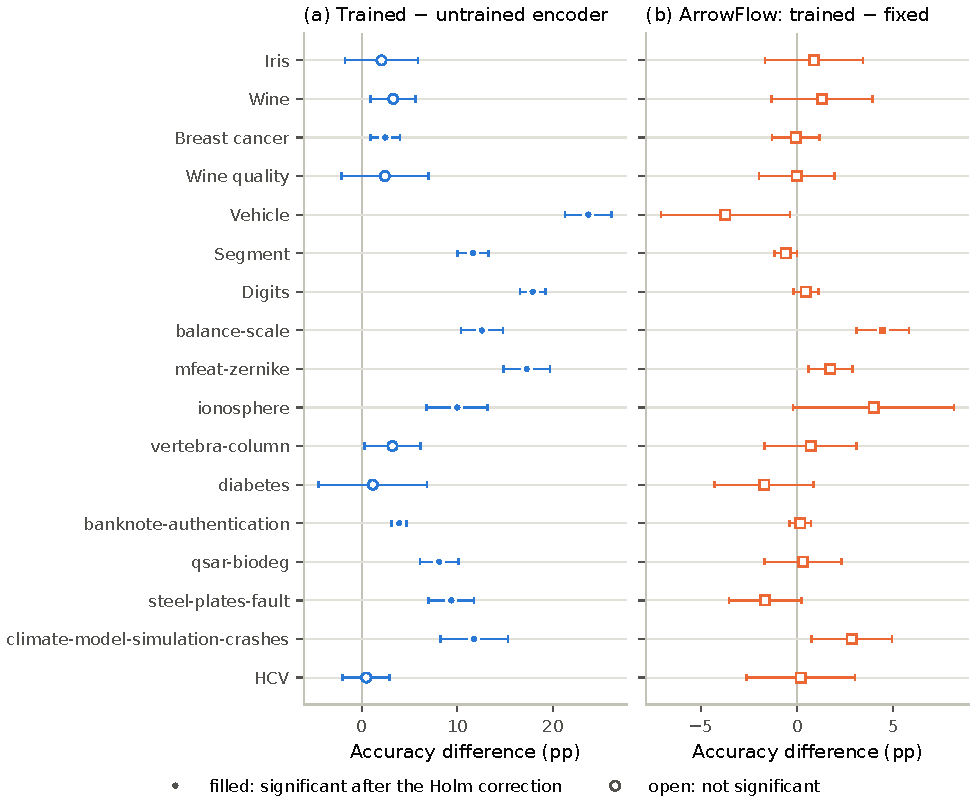
\includegraphics[width=0.92\textwidth]{figures/data/fig9_learned_encoder.pdf}
\caption{\textbf{Can the ranking signal train the encoder?} Accuracy differences, in percentage points, with 95\% intervals (not simultaneous); positive favors the trained encoder. The two panels have different scales. The intervals are not adjusted for multiple comparisons, so an open mark's interval can exclude zero. (a)~The classifier of Section~\ref{sec:learned-encoder}, an encoder network and one ranking layer of class filters, with the encoder trained by the converted motions, minus the same classifier with the encoder left at its random start. At that start, the weights of the encoder's first two layers are drawn uniformly from 0 to 1. Training lowers the mean error over the datasets from 25.5 to 17.2 percent. (b)~ArrowFlow with each view's fixed encoder replaced by the trained encoder network, minus ArrowFlow with its fixed encoder. For every split, both use the configuration that ArrowFlow's own tuning chose on the inner folds of that split's training partition. The swap also drops the polynomial expansion and the projection strategies (Section~S6.4). The mean error falls from 15.5 to 14.9 percent. Marks are circles in panel~(a) and squares in panel~(b). Filled marks remain significant after a Holm correction across the seventeen datasets: 11 in panel~(a) and 1 in panel~(b). The trained encoder has the higher mean accuracy on all 17 datasets in panel~(a) and on 11 of the 17 in panel~(b). The target conversion was developed on twelve of these datasets, all but Wine quality, banknote-authentication, qsar-biodeg, climate-model-simulation-crashes and HCV (Section~S6.2). HCV: hepatitis C virus.}
\label{fig:learned}
\end{figure}


\paragraph{Does the encoder network learn?} We tested the encoder network with one ranking layer of class filters on top, tuned on the same inner folds and scored on the same test sets (Section~S6.3). Trained by the converted motions, it was more accurate than the same network left at its random start on all 17 datasets, significantly so on 11 (Figure~\ref{fig:learned}a). So a discrete ranking signal trains continuous weights without differentiating the sort, as other methods that keep the ranking step exact also do (Section~\ref{sec:related}). The untrained encoder is a weak reference, though. Its first two layers start with weights drawn uniformly from 0 to 1, and its mean error is 25.5 percent, against 17.2 percent after training. The largest gain, 23.7 points on Vehicle, started from an error of 48.7 percent.

Two more contrasts were fixed before the run. Read by its class filters, the trained classifier still trails the tuned MLP. It is ahead on 3 datasets, significantly on none, and significantly behind on 4. Read instead by a nearest-neighbor vote, a single trained encoder with no hidden ranking layer comes close to ArrowFlow, with a mean error of 15.6 against 15.5 percent (Section~S6.3).

\paragraph{Does ArrowFlow gain from it?} We then rebuilt ArrowFlow for every split, with the configuration that ArrowFlow's own tuning chose on the inner folds of that split's training partition. In each view, an encoder network trained on the view's training rows replaced the fixed encoder (Section~S6.4). This also removed the polynomial expansion and the three projection strategies. The views then differed only by their seeds, and no view used linear discriminant coordinates. With the fixed encoder, the rebuild reproduced the stored predictions exactly on the four test sets we checked, at all three fitting seeds (12 fits; Section~S6.4).

With the trained encoder network, ArrowFlow had the higher mean accuracy on 11 of the 17 datasets, significantly on balance-scale, and was significantly less accurate on none (Figure~\ref{fig:learned}b). Its mean error over the datasets fell from 15.5 to 14.9 percent. The rule fixed before the run has two conditions: a higher mean accuracy, and more datasets significantly higher than significantly lower. Both hold, so the rule reads that the trained encoder improves ArrowFlow. A single dataset, balance-scale, meets the second condition, and the conversion was developed partly on it. Across the datasets the gain is not established (post hoc one-sided signed-rank test, $p=0.095$). Left untrained, the same network made ArrowFlow less accurate than the fixed encoder did on 16 of the 17 datasets. So the gain comes from training. Swapping in the network alone makes ArrowFlow worse.

\paragraph{How far does it go?} The trained encoder made ArrowFlow less accurate on 6 of the 17 datasets, by up to 3.7 points on Vehicle, although none of these losses was significant. Every configuration had been tuned for the fixed encoder, which favors the fixed encoder in this comparison. With the trained encoder, ArrowFlow's mean error of 14.9 percent is close to the tuned MLP's 14.6. On balance-scale its error of 1.6 percent is the lowest of all the tuned models. But it still trails the best tuned classical model on 15 of the 17 datasets (Section~S6.4). These comparisons are descriptive, and on balance-scale the lead over the MLP is not significant. The MLP reached its iteration cap before convergence on 331 of its 765 outer fits (Section~S3.2). Against the single trained encoder read by a nearest-neighbor vote, ArrowFlow with the trained encoder is ahead on 15 of the 17 datasets, by 0.67 points on average, and significantly on none (Section~S6.4).
